\documentclass[letterpaper]{article}
\usepackage{aaai}
\usepackage{times}
\usepackage{helvet}
\usepackage{courier}
\usepackage{graphicx}
\usepackage{url}
\usepackage{fancyvrb}

\newcommand{\citenoun}[1]{\citeauthor{#1}~\shortcite{#1}}
\newcommand{\citenounpg}[2]{\citeauthor{#2}~\shortcite[#1]{#2}}

\title{Computational Support for Play Testing Game Sketches}

%\author{Paper \#4\\
%Keywords: game design, logic, scripting
%}
\author{Adam M. Smith$^\star$, Mark J. Nelson$^{\star\dagger}$, Michael Mateas$^\star$\\
$^\star$ Expressive Intelligence Studio, University of California, Santa Cruz\\
$^\dagger$ School of Interactive Computing, Georgia Institute of Technology\\
\texttt{amsmith@cs.ucsc.edu, mnelson@cc.gatech.edu, michaelm@cs.ucsc.edu}
}
\copyrightyear{2009}

\begin{document}
\maketitle

\begin{abstract}

Early-stage game prototypes need to be informative without requiring excessive
commitments. Paper prototypes are frequently used as a way of trying out core
mechanics while leaving them easy to change. Play testing on even these
early-stage prototypes can give an idea of how the rules play out and whether
the game is fun and engaging.  Recently, researchers have proposed using
automated analysis of games to discover additional properties of games, such as
exploits and other gameplay issues.

We propose a lightweight game-sketching approach to give designers access to
insight derived from both human and machine play testing. Using our system,
BIPED, a designer specifies a game's mechanics and maps them to a set of
board-game-like primitives. Games created with BIPED can be played
interactively on a computer as well as automatically analyzed, giving designers
two complementary sources of design backtalk.

In this paper, we describe the language designers may use to sketch games,
how they might use our tool in the two modes of play testing, and how the prototypes
are computationally realized. Additionally, we study using our system to prototype
a game and examine it in human and machine play tests.

\end{abstract}

\section{Introduction}

Prototypes, both physical and computational, are an essential tool in a game
designer's arsenal. In a popular game-design text, \citenoun{Fullerton} defines
a prototype to be ``a working model of your idea that allows you to test its
feasibility and make improvements to it''. At the earliest stages, the designer
can operate purely conceptually, thinking up new mechanics and imagining how
they might interact with each other and the player; but at some point all
designers need to try them out. This has been described as getting
\emph{backtalk} from a design situation: the designer begins with some idea of
how her design should work, but by trying out a prototype, she uncovers unforeseen
new information on how it actually does work~\cite{Schoen:book}. In game
prototyping, that new information can be both in terms of player experience,
observing player's excitement or hesitation to take a critical
action; and in terms of how the game's rule system operates, laying bare
gameplay exploits and additional solutions to counterintuitive puzzles.

Physical prototypes are an early-stage game design and play testing tool, in
which low-fidelity versions of a game's core mechanics are mocked up. Even a
complex real-time videogame can be prototyped using cards, tokens, dice, and
similar physical objects~\cite[ch.\ 7]{Sigman:Gamasutra,Fullerton}. These
prototypes aim to let the designer get backtalk after minimal effort, before
committing to the cost of building a computational prototype (though it may provide
higher-fidelity backtalk). An important aspect of low-commitment techniques is
the ease of exploring related ideas.

There is some gray area between physical prototypes and computational
prototypes as well. One common way of using a computer to run the game's rules
while keeping things lightweight is to use a spreadsheet, either stand-alone or
as a computational aid to physical prototypes. The designer writes the game
rules in a scriptable spreadsheet, and has it update game state as players take
actions~\cite[pp.\ 216, 221, 246]{Fullerton}.  This style of prototyping is
best suited to numerically oriented games, such as physical or economic simulations.
However, many of the elements used in physical prototypes do not
transfer well to spreadsheets. Instead, there are discrete cards and
tokens, and rule systems with many cases and spatial rearrangement of the
tokens, rather than equations that update numerical fields.

We propose a game-sketching approach to provide computational support for the
class of physical prototypes that use board-game like elements to
represent complex videogames. Through this approach, game designers
can access formal analysis afforded by computational approaches while designing
prototypes similar to those made with physical methods. The designer specifies
game state, possible player actions, and state update rules.  Elements of game
state can be mapped on to a simple set of board-game primitives---connected
spaces and tokens---and user actions are mediated by UI affordances such as
clicking and dragging, constituting a fully playable game suitable for early play testing.
Using logical reasoning, we also allow the designer to query formal
properties of their sketch, such as getting examples of possible gameplay
traces resulting in specific outcomes (or using specific means to achieve
these). Our contribution is a technique that supports machine and human play
testing, using a single game-sketch definition, to provide designers with the
best of two complementary sources of backtalk. 

\section{Play testing background}

What can designers get out of play testing, and why would they need both kinds?
We review discussions of human play testing in the game design literature, and
proposals for machine play testing in the artificial intelligence literature,
to provide a background for the kinds of design backtalk that have been
proposed as particular strengths of each approach, especially as applied to
early game prototyping.

\subsection{Play testing with humans}

\citenounpg{ch.\ 7}{Fullerton} has an extensive discussion of early
prototyping and the kinds of design questions play testing with them can
answer. She describes four main stages of prototyping. In the first, the
designer focuses on foundations, looking at only a loose version of the core
mechanics and avoiding filling in details like how many squares a player can
move; the designer self-tests to validate and flesh out the design. In the
second, the focus is on the game's structure, specifying rigid mechanics
such as combat-resolution rules.  The third
stage fills in formal details and tweakable constants, such as starting health level and hit
percentages, as well as minor elaborations on mechanics. In the last stage,
the designer focuses on game flow and understanding how 
features of the game contribute to the play experience.

Implicit in most discussions of play testing is that important elements of
gameplay come from intrinsically subjective human reactions.
\citenoun{theoryoffun} focuses in particular on fun and engagement and their
relation to an individual's process of learning a game's mechanics.
\citenoun{Mirjam:MMO} discuss feedback from paper prototypes testing a game
mechanic derived from personality theory, with play tests focusing on how the
mechanics connect to players' personalities and subjective gameplay
experiences.

\subsection{Play testing with machines}

Although the subjective human experience of games is the key to their success,
designing games involves crafting formal rule systems and understanding how
they operate as well. \citenounpg{ch.\ 12}{SalenZimmerman} discuss emergent
properties of game rules, since a small set of rules might actually imply a
larger set that are not explicitly specified; understanding these implications
can help a designer decide how to revise the game towards its intended subjective
experience. Since the formal properties of game rules are amenable to automated
reasoning, \citenoun{NelsonMateas:FDG09} study what kinds of objective
questions designers would find useful to ask; automatically providing answers
to those questions would free up the designers to focus on more subjective
design issues.

\citenoun{Salge:Sandbox} apply artificial intelligence to play testing, going
as far as to argue that automatic testing can be superior to human 
testing, because human testers instinctively try to play in a balanced and
fair style. An automated agent, by contrast, could look for exploits in the
game rules without preconceived notions of how the game should be
played.

\citenoun{NelsonMateas:AIIDE08} propose that designers prototype their early
rule systems in a formal language, in exchange for which they can receive
abstract gameplay traces. These play traces may illustrate interesting or
undesirable gameplay possibilities that motivate a change, finding early issues
with the game rules before spending time on human play testing (or even writing
code for input and graphics).

\section{System overview}

\begin{figure}
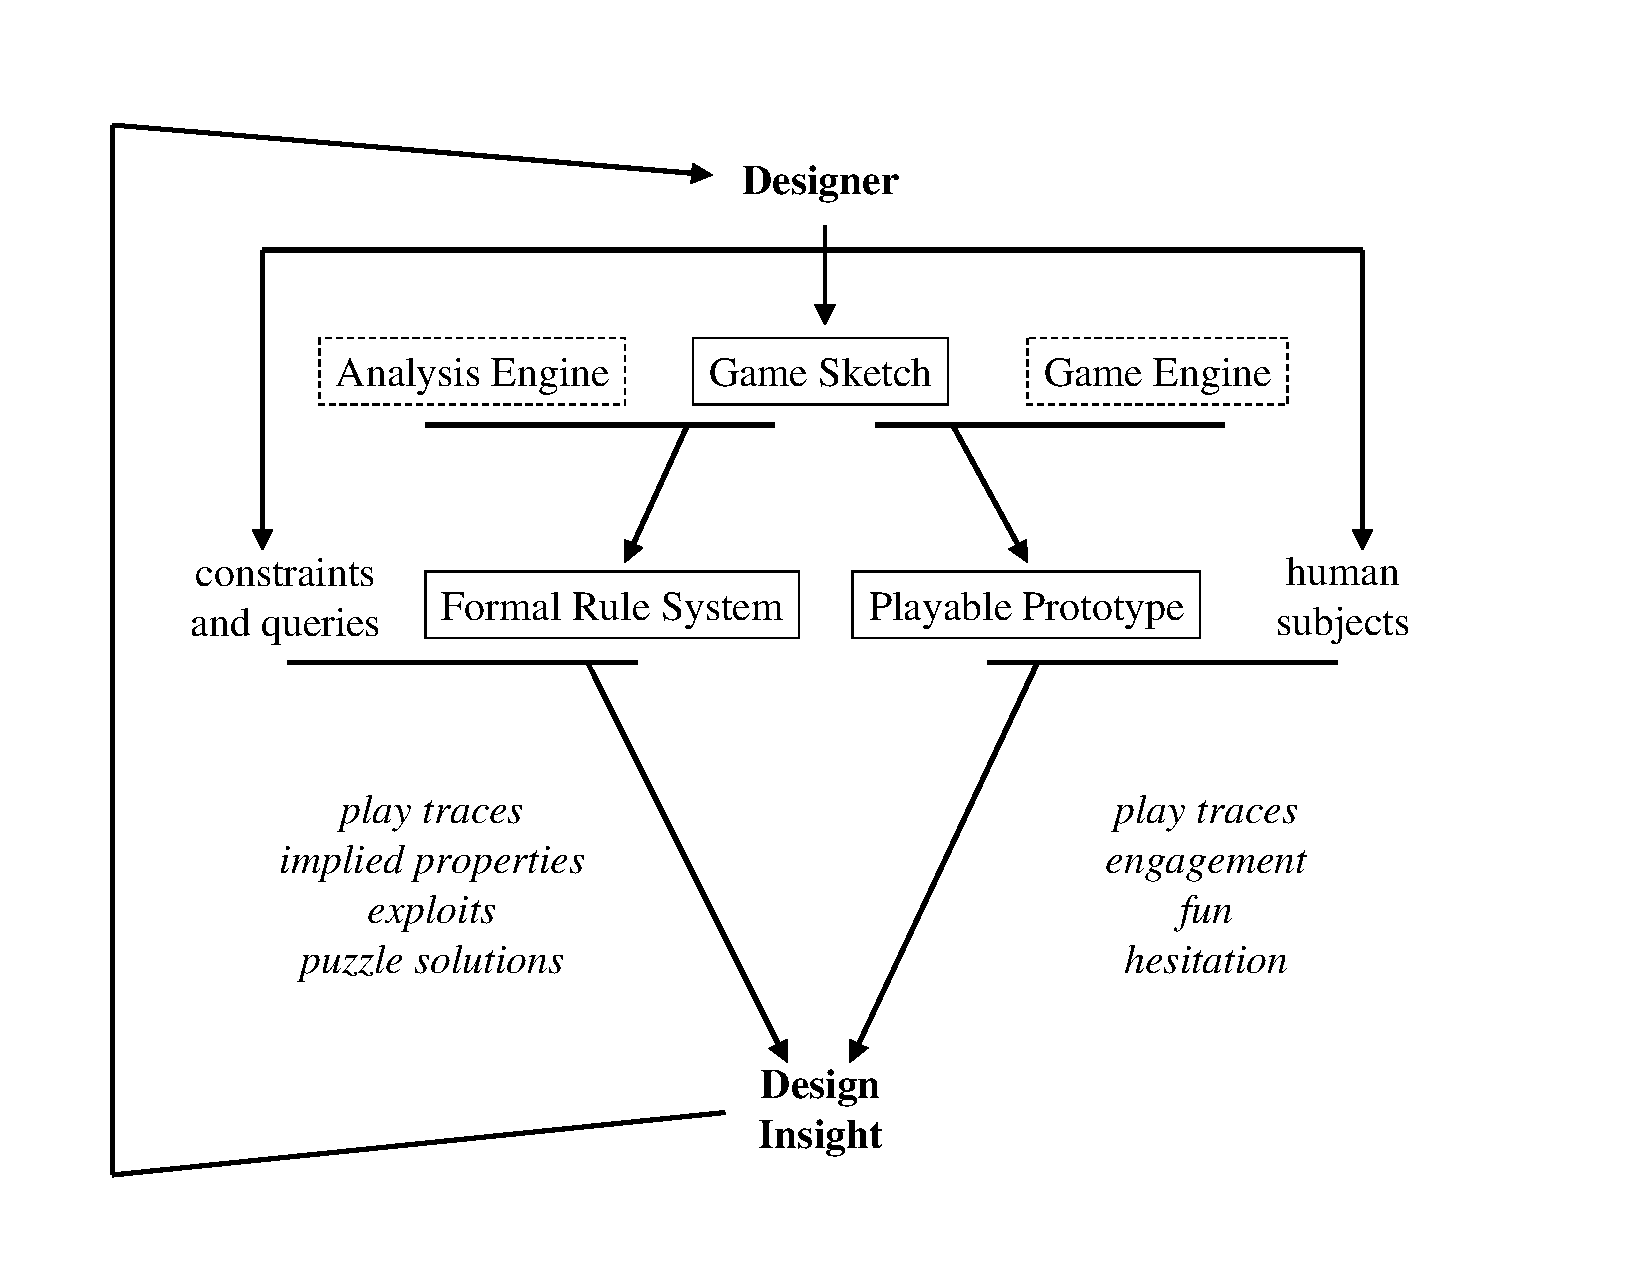
\includegraphics[viewport=0.5in 0.5in 9.5in 8in,clip,width=\columnwidth]{architecture.pdf}
\caption{Architecture diagram for the BIPED system.}
\label{fig:arch}
\end{figure}

The architecture of BIPED, with its dual support for human and machine play
testing, is shown in Figure~\ref{fig:arch}. A designer using our system begins
by writing a game sketch. This sketch is combined with an analysis engine to
produce a formal rule system on which the designer can perform machine play
testing. To do so, she specifies combinations of queries and constraints and
can get back abstract gameplay traces with specific characteristics, determine
implied properties of the rule system, find exploits, and list solutions to
puzzles.  The sketch can also be combined with our game engine to produce a
playable prototype, which, when the designer or human subjects she recruits
play it, can give feedback on more subjective properties of the game, such as
player engagement, fun, or hesitation, as well as traces of actual gameplay.
From these two sources of backtalk, design insight may prompt the designer to
perform another iteration.  We should emphasize that our approach focuses on
early design prototypes, not late-stage prototype implementations of a full
game.

\subsection{Game sketching language}

\begin{figure}
\begin{Verbatim}[frame=single,fontsize=\scriptsize]
agent(pc).
agent(thief).
item(loose_coins).
item(assorted_gems).

game_state(has(A,I)) :- agent(A), item(I).
game_event(drop(A,I)) :- agent(A), item(I).
terminates(drop(A,I),has(A,I)) :- agent(A), item(I).
possible(drop(A,I)) :-
   holds(has(A,I)), agent(A), item(I).
\end{Verbatim}
\caption{Snippet of the game sketch language defining part of an inventory mechanic. The last rule,
for example, says: the game event that an agent drops an item is only possible if the agent has the item, for
any agent or item.}
\label{fig:lang}
\end{figure}

Game sketches are defined in a subset of Prolog (chosen for its clean,
declarative style); an example defining an inventory mechanic is shown in
Figure~\ref{fig:lang}. The designer can use logical predicates and constants to
specify the entities in the game world and their properties. In this example,
there are two agents, the player character and a thief; as well as two items, a bunch
of loose coins and set of assorted gems. Entire levels can be described in a
similar manner, specifying, for example, the rooms of a dungeon and hallways
between them.

A special set of predicates is recognized by the language. These can be used to
specify the dynamic parts of the sketch, organized around \emph{game state} and
\emph{game events}.  The game state is a set of properties that vary over time,
under the influence of game events.  The game engine and analysis engine are
implemented so as to provide a common semantics for these predicates, ensuring
what is possible in the human-playable version is possible in the logical
version and vice versa.  Returning to the example in Figure~\ref{fig:lang}, the
\emph{has} game state specifies, for any agent and item, whether the agent has
that item.  The next rule specifies a \emph{drop} event (for any agent and
item). The following rule gives the event's effect: it terminates the
\emph{has} state (sets it to false). The final rule specifies that a
\emph{drop} event is only possible when the \emph{has} state \emph{holds} (is
true).  Similar, but not shown in this example, are \emph{initiates}, which is
analogous to \emph{terminates} but specifies that an event sets an element of
game state to true; and \emph{conflicts}, which specifies restrictions on when
events can happen simultaneously. The \emph{initially} predicate can also be
used to specify the elements of game state that hold at the beginning of the
game.

\subsection{Interface elements}

\begin{figure}
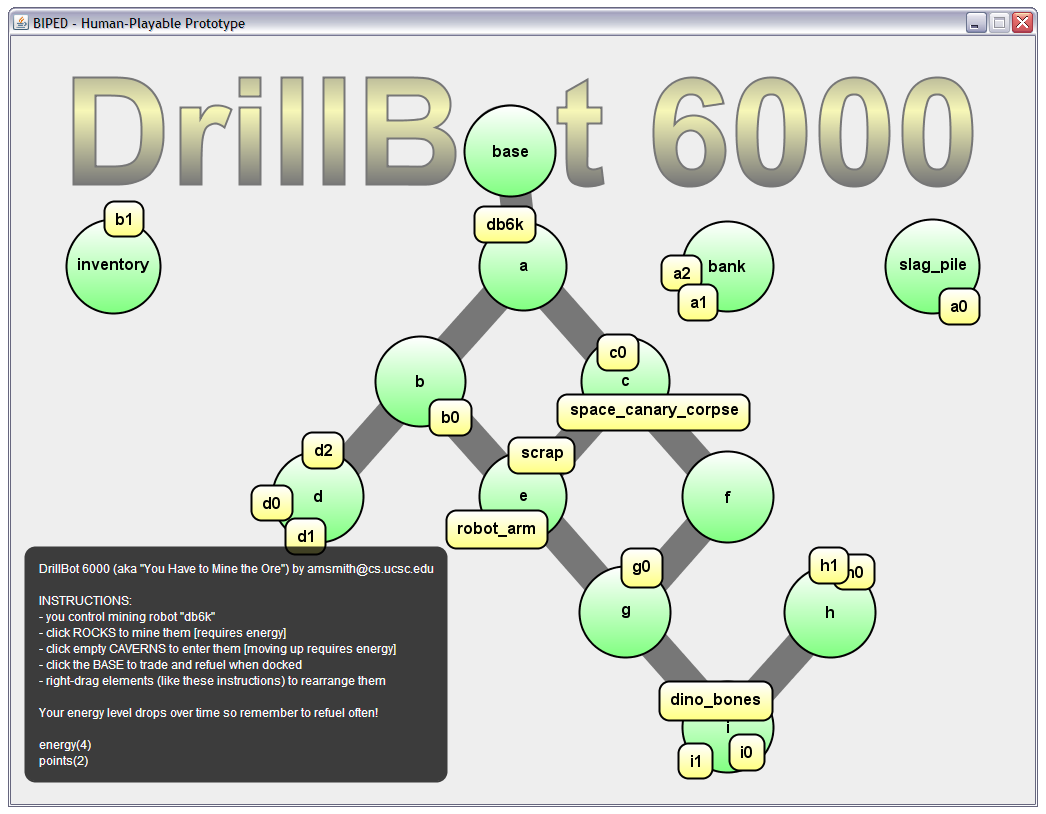
\includegraphics[width=\columnwidth]{db6k_screenshot.png}
\caption{Human-playable prototype for our example game.}
\label{fig:screenshot}
\end{figure}

\begin{figure}
\begin{Verbatim}[frame=single,fontsize=\scriptsize]
ui_title('My adventure game').
ui_space(R) :- room(R).
ui_token(I) :- item(I).
ui_triggers(ui_click_space(R), move_to(R)) :- room(R).
ui_triggers(ui_click_token(I), grab(I)) :- item(I).
\end{Verbatim}
\caption{Bindings from UI elements to a game world.}
\label{fig:bindings}
\end{figure}

To complete the prototype, a set of interactive visual
elements are available to specify a game's playable representation. Based on
the kinds of representations often used in simple physical prototypes, the main
interface elements are clickable tokens and spaces, with optional connecting lines between
spaces. Figure~\ref{fig:screenshot} shows an example of the interface presented
to the player. Figure~\ref{fig:bindings} gives a simple example of setting up
interface elements and connecting them to a game world. In this
code example, there is a visual board space for every room in the game world (as well
as a token for every item).  Clicking on a board space that represents a room
is set to trigger a \emph{move\_to} event in the game world for that room (similarly for
tokens and grabbing of items).

As with actual physical prototypes, there are many ways of using the visual
elements to represent the state of the game world, and mappings need not all be
as direct as in this example. Spaces can instead be used to represent
inventory, with tokens on the space representing items in the inventory; or
they can be buttons, with clicks causing a state change that may be reflected
in a different part of the visual representation; or space and token
combinations can represent turns or phases of the game (just as a physical
dealer token is passed around a poker table). Similarly, connecting lines
need not only represent how tokens can move between spaces; they
might represent other relationships between entities represented by the spaces,
or elements on which a button would operate when pressed.  As a result of this
flexibility, the designer does need to recall that there is no automatic
meaning of the UI elements in terms of the game-world state: instead, it is
their responsibility to give the representation elements game-relevant
semantics.

In addition to the visible elements, our event system is a major
representational tool. Time in the game world logically stands still until an
event happens. The only sources of events are mouse interactions and expiration
of timers. The effect of a living game world can be achieved using a ticker to
create a regular stream of tick events, which can trigger interesting
game-world events. The \emph{ui\_triggers} predicate defines these mappings
from mouse-interaction and timer events to game-world events; it checks to
ensure that it only triggers game-world events if they are \emph{possible} at
the time.

We have been able to mock up a wide range of physical prototypes using this set
of elements, and have avoided introducing a larger range of special-purpose
elements in order to keep the prototypes simple and easy to
modify. We have, however, included a number of aesthetic elements that do not
directly represent game state, such as instructions, title, victory/loss
animations, and background music, that can be used to provide an interpretive
framework for the human play testers. We acknowledge that aesthetics of even
early-stage prototypes can set the mood for the game and impact the subjective
play experience, even if they are not the main focus~\cite{Sigman:Gamasutra}. In
particular, end conditions that support a subjective distinction between good
and bad outcomes are a key feature of games~\cite{Juul:Gameness}.

\subsection{Supporting play testing}

To play-test games created using BIPED, the designer may begin with either
machine or human testing; we have found that each process informs the
other, so alternating between them may be useful.

Human play testing often begins with self-testing. The designer loads a game
definition that she has created into the game engine, and is presented with an
initial playable game. Even before mechanics are fully specified, it is often
gratifying to see on-screen a level previously only described in the abstract.
As the mechanics of a paper prototype are added to the first computational
prototype, many design decisions have to be made to create the desired rigid
rule system. A lightweight cycle of revision followed by self-testing can allow
the designer to quickly flesh out these rules while playing the game
themselves, giving a first glimpse at the gameplay possibilities afforded by
their sketch.

When testing with others, it is important to formalize any parts of the game
that the designer may have been keeping in their head during self-testing.  By
utilizing timers, on-screen instructions, and background music, the designer
can externalize the desired dynamics and mood of the game (\emph{e.g.}\
fast-paced and frenzied). Human play testing is best mediated by the designer,
who can then observe player engagement and hesitation, as well as make verbal
clarifications. Because playable prototypes from BIPED are user-tweakable,
standalone sketches, however, they can be sent to and played by remote individuals
as well (unlike physical prototypes or computational prototypes with extensive
dependencies).

\begin{figure}
\begin{Verbatim}[frame=single,fontsize=\scriptsize]
happens(fires_at(jack,right),0).

display_to(time(1),jill,health(2),enemies_at(right)).
display_to(time(1),jill,health(2),self_at(left)).
display_to(time(1),jack,health(1),enemies_at(left)).
display_to(time(1),jack,health(1),self_at(right)).

happens(fires_at(jill,right),1).
happens(frags(jill,jack),1).

display_to(time(2),jill,health(2),enemies_at(right)).
display_to(time(2),jill,health(2),self_at(left)).
\end{Verbatim}
\caption{Partial trace from a multiplayer shooter game prototype, illustrating
events and game state over time.}
\label{fig:trace}
\end{figure}

Play testing with humans is a well established practice; in contrast, play
testing with machines is a relatively new, speculative idea. Thus, we have
opted to focus on support for extracting gameplay traces, because these seem to
be strongly tied to player experience (as opposed to generating game-playing
agents).

A designer can specify scenarios and conditions, and the analysis engine will
provide her with gameplay traces (if any exist) starting from those scenarios
and meeting those conditions. Figure~\ref{fig:trace} shows a short excerpt of a
trace from a multiplayer shooter prototype, in which an agent, interestingly,
inflicts damage on himself. To look for an exploit, the designer might ask for
traces starting in a particularly tricky scenario, which end in victory only a
few timesteps later. If any traces exist, the designer has a specific example
of the behavior to forbid in the game rules; if not, the engine has proved that
no such exploit is possible (which would be difficult to determine with
certainty using only human play testing). In cases where there are many
uninteresting traces, the designer can restrict the conditions in order to
``zoom in'' on more plausible gameplay. Alternatively, the designer can run
experiments in which the scenario and conditions are held constant, and some
element of the rules is changed. This gives the designer backtalk regarding a
possible rule change rather than more detailed inspection of a particular rule
set.

\subsection{Implementation}

Our implementation is primarily split between two engines. The game engine,
supporting human-playable prototypes, was implemented in the Scala programming
language, which targets the Java Virtual Machine for easy redistribution of
games. The rules of a particular game, implemented in Prolog, are interpreted
using jTrolog,\footnote{\url{https://jtrolog.dev.java.net/}} a Prolog engine
for Java, so game sketches can be modified by end users without recompilation.
The game engine executes the game rules by advancing time in response to UI
events, querying Prolog to find whether visual elements have changed
(\emph{e.g.}\ whether tokens have moved), and which elements of game state hold
on the next time step.

The analysis engine, supporting the construction of complete formal rule
systems, was implemented in
Lparse/Smodels,\footnote{\url{http://www.tcs.hut.fi/Software/smodels/}} an
answer-set-programming toolchain. Building on the work of
\citenoun{NelsonMateas:AIIDE08}, we used a representation of game worlds in the
event calculus, a logical formalism for reasoning about time, and designed the
declaration of game state and game events so they map directly onto
event-calculus fluents and events. A compiler written in Prolog translates the
game-sketch definitions into answer-set programs usable by Lparse. Additionally,
a small Lparse ``game engine'' ties the rest of the game sketch (excluding UI)
into the event-calculus semantics.  The analysis engine is also responsible for
checking that a game sketch is complete (defining a minimal set of required
predicates) and checking any additional designer-specified static properties
(\emph{e.g.}\ there are no rooms in the level description without an adjoining
hallway).

An interesting result of this translation is that when the analysis engine is
looking for traces, it treats time as a symbolic constraint rather than
simulating game worlds forward in time. In this way, it is as easy to put
constraints on initial conditions as it is on end conditions, or on any point
in between. In the game engine behind human-playable prototypes, logical time,
while discrete, behaves much more intuitively, advancing step by step in
response to timers and human interaction (effectively finding a single trace).

\section{Example prototype}

To exercise play testing with BIPED, we created \emph{DrillBot 6000}
(previously illustrated in Figure~\ref{fig:screenshot}).  In this game, the
player moves a mining robot through underground caverns, drilling out rocks of
mixed value, while managing energy usage by periodically returning to the
surface to refuel and trade items. This game was designed as if to be an early
prototype version of the popular Flash game \emph{Motherload} from XGen
Studios.\footnote{\url{http://www.xgenstudios.com/play/motherload}} Our game
focused on the core mechanics: moving around underground, mining, and refueling
(whereas \emph{Motherload} includes shopping for upgrades and story elements).

\subsection{Game mechanics}

To describe the mechanics of the \emph{DrillBot 6000} game world, our 
sketch definition asserts that \emph{position} and \emph{energy} are elements
of game state (that apply to the one robot), and that subterranean rocks can be
\emph{present} in a cavern, \emph{bagged} in the robot's inventory, or
possibly \emph{banked} after trading. In terms of game events, we allow
mining of rocks, moving up or down between caverns, refueling, trading rocks,
and spontaneous energy drain. The game sketch also defines the consequences of
these events, and when they are possible. For example, the
\emph{mine} event for a rock \emph{initiates} the \emph{bagged} state for
that rock, \emph{terminates} its \emph{present} state, and drains a unit
of \emph{energy}. This \emph{mine} event is \emph{possible} if: the rock
is \emph{present}, the location of the rock is reachable from the robot's
current \emph{position}, and the robot has \emph{energy}. The rigid rules
for other game events are defined similarly. Finally, the definition asserts
initial conditions: the robot starts fully energized at the base, and all rocks
are present.

\subsection{UI bindings}

While the game mechanics described above are enough to allow machine play
testing, for human testing we needed to expose the abstract game world to
the player. Caverns are mapped to board spaces, and
the up/down links between caverns are visualized with connecting lines.
Individual tokens represent the minable rocks, and a special token represents
the robot itself. The UI event of clicking a rock's token is bound to the
\emph{mine} event for the corresponding rock. Likewise, clicking a cavern's
space is bound to either a \emph{move\_up} or \emph{move\_down} event to that
cavern. These bindings are expressed concisely without need to reiterate the
necessary conditions (\emph{e.g.}\ the
proper \emph{move\_up} or \emph{move\_down} event is selected by virtue of
the game-world definition of when these events are \emph{possible}).

We bound the position of rock tokens to cavern spaces using the abstract level
definition and the \emph{present} status of the rock to select a space. When
rocks are not present, the player should have a way of knowing the rock's
\emph{bagged} or \emph{banked} status. The additional spaces called
\emph{inventory}, \emph{bank}, and \emph{slag\_pile} are used as the location
for rock tokens that are no longer present but have differing bagged or banked
states (valueless rocks cannot be banked, and their tokens are sent flying to
the slag pile with a quick animation). Spaces themselves are anchored to the
board with an optional predicate; these positions were consciously set to
portray the directionality of links between caverns.

To give our prototype an element of the time pressure present in
\emph{Motherload}, there is a ticker for which the tick event is bound to the
game world's \emph{drain} event, draining a unit of the robot's energy.
Thus, robot energy drains at a regular pace, but faster when the player
actively triggers game-world events that consume energy. Energy is replenished
by clicking on the base's space, which triggers the game-world \emph{refuel} and
\emph{trade} events simultaneously.

A game definition also specifies several non-interactive elements.
A large title and background music set the tone for a lively real-time mining
game. On-screen, written instructions lay out both the premise of the game and
explain how the player can use the mouse to take actions in the world of rocks,
caverns, and a robot. Some elements of game state not mapped to spaces and
tokens are depicted textually, in this case energy level and score.
Finally, when the game determines that no additional actions are possible, a
few tokens fly onto the screen to announce the game's outcome.

\subsection{Human play testing}

As suggested by \citenounpg{p.\ 252}{Fullerton}, since we were testing the
foundations and structure of the game, we primarily tested \emph{DrillBot
6000} by self-testing and testing with confidants. Self-testing revealed that
our early iterations had allowed unintended gameplay; for example, you could
mine a rock at arbitrary distances. Additionally, we found the first version of
the game too simple, and decided to add several additional rocks and caverns.
When testing with others, one tester initially felt pressured by the speed of
the automatic energy drain. While we could have adjusted the speed of energy
drain or the maximum energy level, at this stage of the prototype we were
interested in more foundational questions, rather than
game balancing. To get feedback on the game's other mechanics, we showed the
tester how to convert the game to a turn-based one by removing the ticker.  All
three testers claimed to enjoy the game, and could reach rocks at the deeper
levels after some practice. Interestingly, no testers related to the game as a
puzzle or path-planning challenge, even in turn-based mode; all focused instead
on the action aspect of the game motivated by the continuously draining energy.

\subsection{Machine play testing}

While human play testing validated that the game's basic concept was
interesting, BIPED allowed us to turn to machine play testing to ask more
detailed questions that would have been tedious or impossible to test with
human testers. Because players focused on improving their speed, in 
machine play testing we decided to look at the limit case, corresponding to a
player that could execute several actions without incurring any time-based
energy drain (which was possible but difficult with our timer settings). This
would allow us to focus on the energy cost of mining and moving as the
limiting factors, effectively discovering speed runs.

In one experiment, we looked for gameplay traces that maximized the number of
treasures the robot could bank by the end of a fixed number of timepoints.  In
15 timepoints, we found that the ideal player could bank up to five valuable
rocks. Then we asked about a player who would never refuel, wondering if
this would place some rocks out of reach. Over this game length we found that
the ideal player could still bank five valuable rocks, indicating that
refueling is needed relatively infrequently. This was interesting, because our
human testers refuelled quite often, as a hedge against energy drain,
indicating that they were much more cautious with managing energy than strictly
necessary.

In the setup for this experiment, when looking at general gameplay traces, we
found undesirable traces in which several rocks were mined simultaneously.
This revealed that we had not completely specified when game actions
should conflict. That issue was not revealed in human testing,
because the UI bindings happened to make it impossible to mine several rocks at
the same time (which would not be the case if mining had been tied to clicks on
spaces instead of on tokens). Finding that this design choice was incompletely
specified both forced us to think about what mechanics we actually did want,
and avoided the persistence of a UI-masked bug that could reappear
in later prototypes.

In another experiment, we looked at a few properties of the level's design.
One question involved asking how many caverns a player could explore in a
given interval (where the robot starts and ends in the base). This query is
particularly tedious to answer through human play testing, since it would
require trying a vast number of possibilities. It also goes beyond simple graph
search, because it takes into account the effects of time-varying presence of
rocks due to mining. In 15 timepoints, a player can explore up to eight caverns
before returning to the base. Making what we thought would be a radical change
to the level's design, we added a direct link from the base down to the deepest
cavern in the level. Running queries for reachable caverns and banked rocks
again, we were surprised to find this change made no difference in the
properties of the optimal play-through.

\section{Conclusions and future work}

We have proposed a computational prototyping approach to combined support for
human and machine play testing of early-stage game sketches. This approach has
been cached out in BIPED, a tool that uses declarative game descriptions to
produce both standalone, playable games and formal rule systems that admit
automatically finding gameplay traces with specific properties (while
minimizing design commitments, yet allowing sufficient interpretive affordances
to support useful human play testing). We explored the process of designing with BIPED
by prototyping \emph{DrillBot 6000}, an action-oriented game in the style of
\emph{Motherload}. In doing so, we illustrated the
synergy of human and machine play testing for insight into the game's
design.

The semantics of our game-sketching language are based on a knowledge
representation which is optimized for designer exploration, while the syntax
used here was chosen in large part to minimize the distance to the two
declarative reasoning engines involved. In future work, we intend to address
the language's accessibility, particularly to game designers without a
logic-programming background; it is best to think of the language presented
in this paper as an intermediate representation.  In addition, future work
should investigate other reasoning backends for the analysis engine with better
scaling and numeric processing capabilities.

Several miscellaneous improvements to this approach could be unified in a
game-design ``workbench'' that bundles all the tools necessary for a designer to
carry out exploratory game design, including a better query language paired
with more intuitive visualization of results. Additionally, such a tool should
provide a more fluid way of modifying a game's mechanics than editing a logic
program.

A tool like BIPED is an interesting target platform for
automated game generation research (whether aiming to create whole new
mechanics or just tweaking level designs). Moving beyond generation, the
addition of detailed instrumentation to the human-playable prototypes would
admit collecting enough information from human play testers to inform the
analysis used in an intelligent game-design agent that might learn from
how humans play the games it produces.

Finally, an open problem is how to extend the human--machine play
testing approach to later stages of the game-design process. For now, our
approach is focused on allowing designer-programmers to take large creative
leaps by getting rich feedback from simple, early-stage prototypes.

{\small
\bibliographystyle{aaai} \bibliography{references}
}

\end{document}

